% Technical Report — Human Safety Monitoring System (INaAI 2026, Domain 1)
% Kompilasi: pdflatex technical_report.tex  (atau unggah ke Overleaf).
% Butuh: confusion_matrix_normalized.png di folder yang sama.
\documentclass[10pt,a4paper]{article}
\usepackage[margin=1.5cm]{geometry}
\usepackage[T1]{fontenc}
\usepackage{lmodern}
\usepackage[dvipsnames]{xcolor}
\usepackage{graphicx}
\usepackage{booktabs}
\usepackage{enumitem}
\usepackage{titlesec}
\usepackage[hidelinks]{hyperref}

\definecolor{accent}{HTML}{B8860B}
\titleformat{\section}{\normalfont\large\bfseries\color{accent}}{\thesection.}{0.4em}{}
\titlespacing{\section}{0pt}{6pt}{3pt}
\setlist[itemize]{leftmargin=1.2em,itemsep=1pt,topsep=2pt}
\setlength{\parindent}{0pt}\setlength{\parskip}{3pt}
\pagestyle{empty}
\newcommand{\code}[1]{\texttt{\small #1}}

\begin{document}

{\LARGE\bfseries Human Safety Monitoring System --- Technical Report}\\[2pt]
{\small INaAI Competition 2026 $\times$ IT Del $\cdot$ AI Engineer Track $\cdot$ Domain 1: Human Safety Monitoring (Computer Vision)}\\
{\small William Panjaitan $\cdot$ \url{https://github.com/20WilliamPanjaitan/Human-Safety-Monitoring-System} $\cdot$ Juni 2026}\\[-4pt]
{\color{accent}\rule{\linewidth}{0.8pt}}

\section{Problem \& Scope}
Sistem monitoring keselamatan manusia berbasis kamera untuk area konstruksi. Diimplementasikan \textbf{4 dari 5} modul (minimum 3): \textbf{person detection}, \textbf{person tracking}, \textbf{PPE detection} (helmet/vest/mask), dan \textbf{people counting}. Face recognition sengaja tidak diimplementasi (privacy/PDP-by-design + batas waktu). Satu model \textbf{YOLOv8s multi-class (7 kelas)} menggerakkan semua modul, disajikan lewat \textbf{inference endpoint FastAPI} (ONNX Runtime untuk gambar, PyTorch untuk tracking) dan dashboard Streamlit. Target metrik mAP@0.5 $\geq$ 0.50 (go/no-go) --- tercapai \textbf{0.78}.

\section{Data}
Dataset \textbf{Construction Site Safety} (Roboflow Universe, lisensi \textbf{CC BY 4.0}). 10 kelas asli di-\textit{remap} ke 7 kelas relevan (\textit{Person, Hardhat, NO-Hardhat, Safety-Vest, NO-Safety-Vest, Mask, NO-Mask}) via \code{remap\_labels.py}; kelas Safety-Cone/machinery/vehicle dibuang. Split memakai bawaan Roboflow \textbf{2605/114/82} (train/val/test). Kebocoran diaudit \textbf{2 lapis} (\code{check\_leakage.py}): \textbf{0 duplikat byte-identik (MD5)} antar split; namun \textbf{19 scene video tersebar antar split} (frame dari klip sama ada di train \& test) $\rightarrow$ mAP test sedikit optimistis. Dilaporkan jujur sebagai limitasi, bukan di-\textit{re-split} (yang akan memaksa re-training di window 22,5 jam). Ketujuh kelas muncul di split test; label diverifikasi visual (\code{sanity\_check.py}).

\section{Model \& Training}
\textbf{YOLOv8s} (Ultralytics 8.3.0), transfer-learning dari bobot COCO. Dilatih di Google Colab \textbf{Tesla T4}, \textbf{50 epoch}, imgsz 640, batch 16, \textbf{seed 42} (random/numpy/torch + cudnn.deterministic). Augmentasi: mosaic + close\_mosaic=10, HSV jitter (h .015/s .7/v .4), scale .5, translate .1, fliplr .5, flipud 0. Bobot final \code{weights/best.pt} (MD5 2bdce55a\ldots), diekspor ke \textbf{ONNX} untuk inference CPU yang lebih ringan; parity deteksi ONNX$\leftrightarrow$PT terverifikasi (5/5 identik kelas+conf@2dp). Provenans lengkap di \code{report/MODEL\_PROVENANCE.md} (termasuk run lokal 5-epoch yang di-abort \& dibuang).

\section{Evaluation}
Eval reproducible (\code{eval.py}, seed 42, hasil identik antar-run) pada split test:

\begin{center}\small
\begin{tabular}{cccc}
\toprule
\textbf{mAP@0.5} & \textbf{mAP@0.5:0.95} & \textbf{Precision} & \textbf{Recall}\\
\midrule
0.778 & 0.456 & 0.883 & 0.733\\
\bottomrule
\end{tabular}\\[3pt]
\begin{tabular}{lccccccc}
\toprule
\textbf{Kelas} & Person & Hardhat & NO-Hardhat & Safety-Vest & NO-Safety-Vest & Mask & NO-Mask\\
\textbf{AP@0.5} & 0.843 & 0.879 & 0.562 & 0.857 & 0.786 & 0.761 & 0.755\\
\bottomrule
\end{tabular}
\end{center}

\textbf{Kenapa mAP, bukan accuracy?} Deteksi tak punya ``accuracy'' tunggal: tiap gambar punya jumlah objek berbeda dan kualitas lokalisasi (IoU) penting. mAP mengintegrasikan kurva precision--recall lintas ambang confidence dan IoU per kelas --- menangkap \textit{missed detection} dan \textit{false alarm} sekaligus. Accuracy (benar/total) tak terdefinisi untuk jumlah box yang variabel dan akan menutupi ketimpangan kelas (mis. kelas NO-* yang jarang). \textbf{Insight confusion matrix} (ternormalisasi): Hardhat$\leftrightarrow$NO-Hardhat nyaris tak pernah tertukar (silang 0.02) --- saat model bilang ``no-helmet'', jarang itu false alarm; error dominan adalah \textit{miss$\rightarrow$background} (Person 0.35, NO-Hardhat 0.44), yaitu under-deteksi objek kecil/jarang, \textbf{bukan} salah klasifikasi safety-critical. Ini mode kegagalan yang diinginkan auditor: cenderung ``kelewat deteksi'', bukan ``keliru menyatakan patuh padahal melanggar''.

\begin{center}
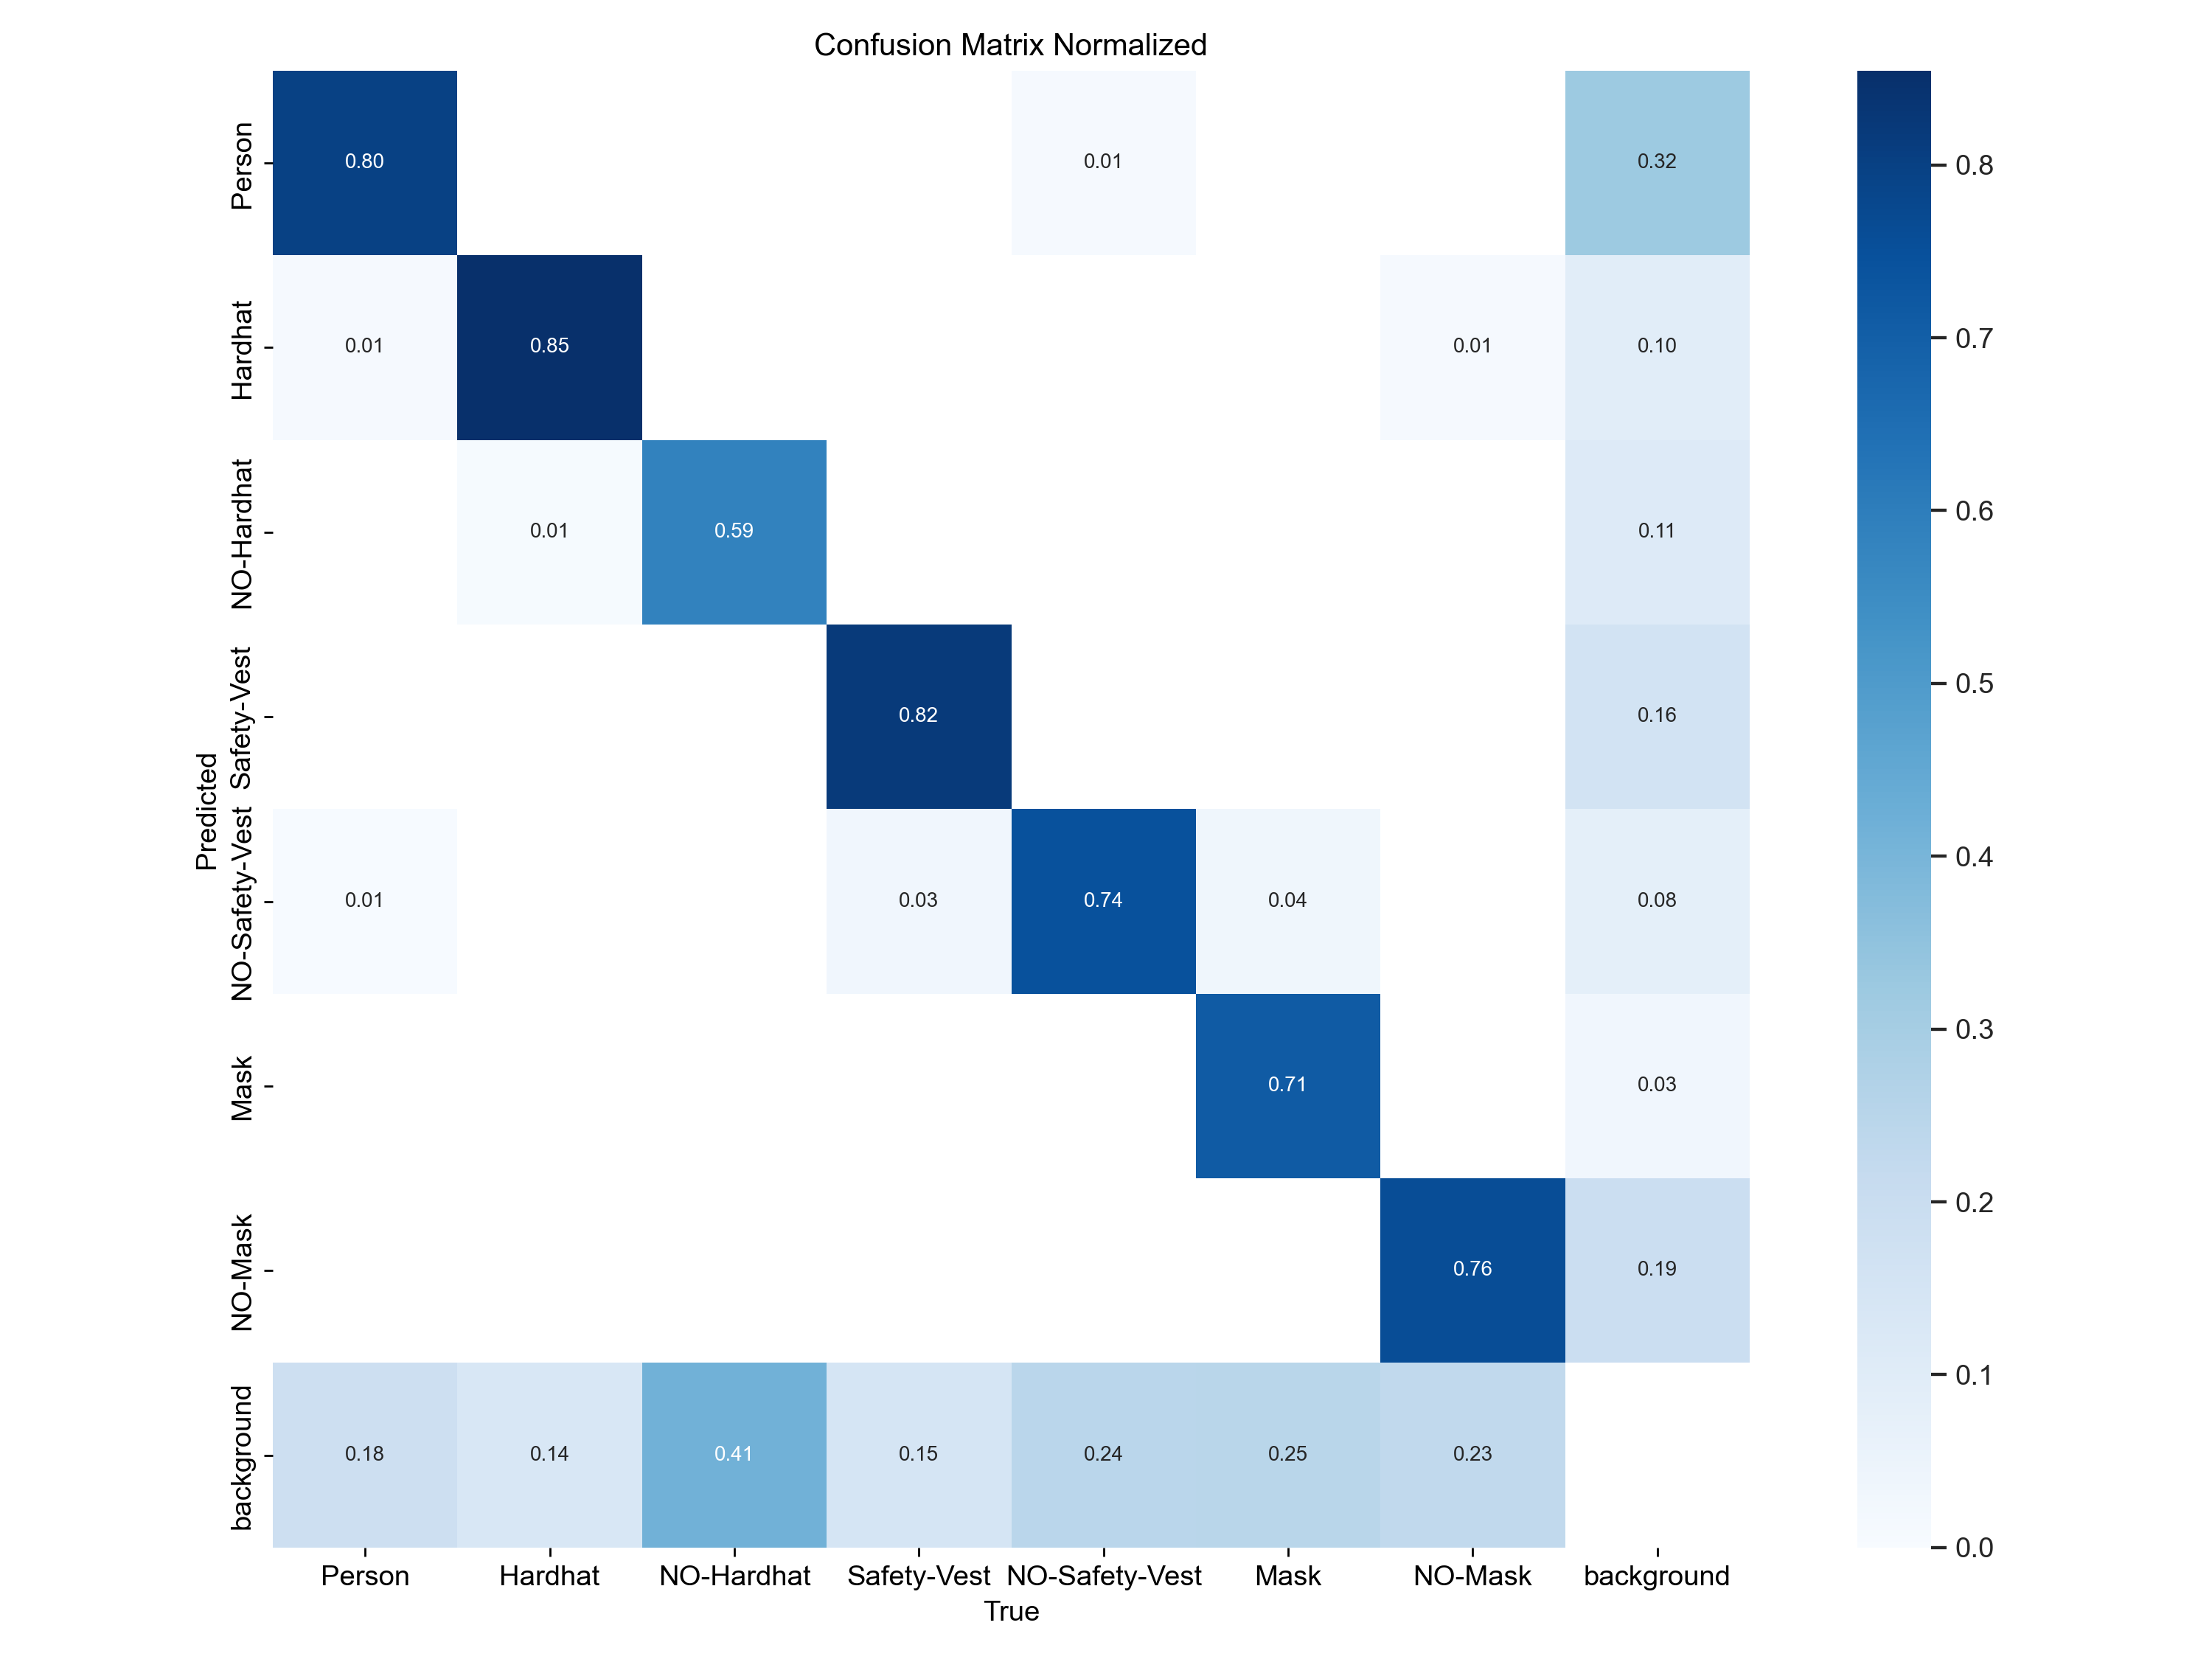
\includegraphics[width=6.6cm]{confusion_matrix_normalized.png}\\
{\footnotesize\itshape Gambar 1. Confusion matrix ternormalisasi (split test).}
\end{center}

\section{System Design}
Satu \textit{core} bersama (\code{app/}) dipakai identik oleh REST API dan UI:
\begin{itemize}
\item \textbf{Detector}: wrapper YOLOv8 (ONNX/PT), di-load sekali, \textit{lazy} saat request pertama (startup ringan).
\item \textbf{PPE logic}: asosiasi PPE$\leftrightarrow$person via \textbf{containment} (fraksi box PPE di dalam box orang), \textbf{bukan IoU} --- IoU gagal untuk PPE kecil vs box orang yang tinggi. Vonis pakai \textbf{bukti positif kelas negatif} (NO-Hardhat/NO-Safety-Vest): status 3-nilai \textit{ok/violation/unknown}. \textit{violation} butuh box NO-* yang overlap; sekadar PPE tak terdeteksi $\rightarrow$ \textit{unknown} (hindari pelanggaran palsu). Wajib = helmet+vest; mask dipantau, tak wajib. Multiple-violation + \textbf{severity} (none/low/high) + agregat \code{summarize()} per-frame (Extraordinary 1).
\item \textbf{Tracking}: \textbf{ByteTrack} (Ultralytics), tuned (\code{track\_buffer=60} utk okulasi singkat, \code{match\_thresh=0.85} kurangi ID-switch); ID stabil antar-frame, jumlah ID unik = people counting versi video.
\item \textbf{Counting}: per-gambar (jumlah box) \& per-video (track\_id unik).
\end{itemize}
\textbf{API} (FastAPI): \code{/health /detect /ppe /count /track /annotate}, tiap respons memuat \code{latency\_ms}, error handling 400/415/500. \textbf{Latency} (CPU lokal): detect $\sim$114 ms, ppe $\sim$116 ms (p50, $<$500 ms target); track klip 9,6 dtk $\rightarrow$ 8,8 dtk (vid\_stride 2, imgsz 480). \textbf{Visualisasi}: \code{/annotate} menggambar box berwarna-kepatuhan (hijau patuh / merah pelanggaran / kuning unverified) + label kelas\&conf; dashboard Streamlit menambah UI interaktif termasuk tab \textit{Robustness Test}. \textbf{Deployment}: dikemas Docker (torch CPU-only) dan di-deploy ke \textbf{Railway} sebagai endpoint publik HTTPS (URL di README); \code{smoke\_test.py} memvalidasi semua endpoint + error-case.

\section{AI Usage Log}
\textbf{Tools.} Claude Code (Anthropic, \textbf{Opus 4.8}) --- asisten coding agentic; Ultralytics YOLOv8 \textbf{8.3.0} (train/inference/val); ByteTrack (built-in Ultralytics). \textbf{Tidak} ada synthetic data atau golden eval hasil LLM (semua metrik dari training/eval nyata), jadi aturan review 30\% tak berlaku.

\textbf{Pola.} Agentic/multi-step: scaffolding, generate kode, debugging, refactor ke production-quality --- tiap perubahan di-review \& diverifikasi manual. \textbf{Prompt utama Fase 2:} (i) bangun dashboard Streamlit modern di atas modul yang ada; (ii) jalankan uji edge-case Tahap 7 + generate aset/laporan; (iii) integrasikan edge-case sebagai tab Robustness di UI; (iv) uji tab di browser nyata; (v) analisis repo $\rightarrow$ dokumen struktur per-file; (vi) audit kelengkapan vs rubrik; (vii) siapkan deployment Docker (Render$\rightarrow$Railway) \& perbaiki kegagalan ABI cv2/NumPy; (viii) tulis report ini. \textbf{Verifikasi \& judgment:} menolak/menyesuaikan saran AI --- mendiagnosis mismatch opencv-headless 4.10 vs NumPy 1.x lalu pin 4.9.0.80; memperbaiki Streamlit \code{use\_container\_width}$\rightarrow$\code{use\_column\_width} (v1.37). Semua kode dijalankan \& diuji (\code{ppe\_demo.py} 8/8 unit, \code{smoke\_test.py} semua endpoint PASS, eval reproducible). History prompt lengkap di \code{AI\_USAGE\_LOG.md}.

\section{Limitations (disadari)}
\begin{itemize}
\item \textbf{Scene leakage}: 19 scene video tersebar antar split $\rightarrow$ mAP test sedikit optimistis (diukur \& diungkap).
\item \textbf{Kelas negatif jarang}: NO-Mask/NO-Hardhat recall terendah (instance sedikit, objek kecil) --- diagonal confusion NO-Mask 0.39.
\item \textbf{Asosiasi crowd}: 1 box PPE bisa di-claim $>$1 orang yang overlap (simplifikasi diterima); NMS padat bisa under-count.
\item \textbf{Tanpa ReID sejati}: ByteTrack berbasis gerak (track\_buffer $\approx$ 2,4 dtk @25 fps); ID bisa berubah setelah keluar-frame lama ($>\!\sim$3 dtk) --- ReID appearance-embedding belum ada.
\item \textbf{Robustness sintetis}: low-light = brightness global $\downarrow$ (model terbukti robust, kemungkinan dari HSV-value aug); noise/blur malam nyata belum diuji. Far/small menurunkan deteksi PPE ($\rightarrow$ unverified, bukan pelanggaran palsu).
\item \textbf{Tanpa face recognition}: sengaja di-descope demi privacy/PDP-by-design \& waktu; alerting berbasis identitas di luar scope.
\item \textbf{Compute free-tier}: CPU-only; \code{/track} klip panjang berat memori (demo pakai klip pendek); ada cold-start pada request pertama.
\end{itemize}

\end{document}
